% Section content template for individual Educative lessons
% This file contains the actual content for a specific section
% Generated from Educative API section content

% Section: Requirements of Yelp’s Design
% Section ID: 4552284171665408
% Section Slug: requirements-of-yelps-design
% Generated: 2025-12-07T23:22:06.508978

\subsection{Requirements}\label{xp9DHV3j5tUq_O5nZNce_}
\\
Let's identify the requirements of our system.

\subsubsection{Functional requirements}\label{7pSile0Uf1mzWuOxaFryD}
\\
The functional requirements of our systems are below:

\begin{itemize}
\item
\protect\phantomsection\label{L1DY7Tr-gkzT6kWE4M2Zg}
\textbf{User accounts}: Users will have accounts where they're able to perform different functionalities like log in, log out, add, delete, and update places' information.
\end{itemize}
\begin{quote}
\textbf{Note:} There can be two types of users: business owners who can add their places on the platform and other users who can search, view, and give a rating to a place.
\end{quote}
\begin{itemize}
\item
\protect\phantomsection\label{00FiokrTXZrO8KLUYq2po}
\textbf{Search}: The users should be able to search for nearby places or places of interest based on their GPS location (longitude, latitude) and/or the name of a place.
\item
\protect\phantomsection\label{SoK2Nsna5o2vtwHWTkbxs}
\textbf{Feedback}: The users should be able to add a review about a place. The review can consist of images, text, and a rating.
\end{itemize}

\begin{figure}[htbp]
 \centering
 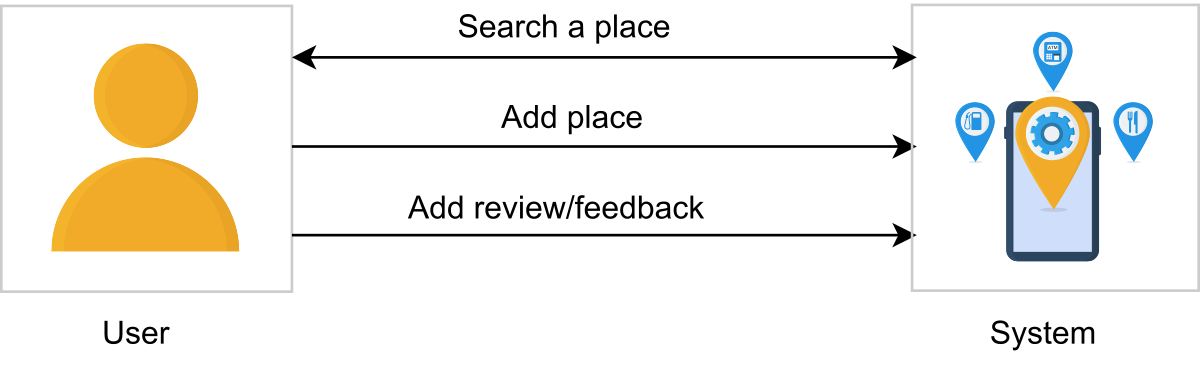
\includegraphics[width=0.5\textwidth]{Images/chapter_29/section_4552284171665408/5804046921498624.png}
 \caption{Functional requirements}
\end{figure}

\subsubsection{Non-functional requirements}\label{N4cUEmhAiBt7L8f7wRehH}
\\
The non-functional requirements of our systems are:

\begin{itemize}
\item
\protect\phantomsection\label{T9Z8_KZ8_BT_RIovQqdSg}
\textbf{High availability}: The system should be highly available to the users.
\item
\protect\phantomsection\label{y7q-xCZLjrT5jU84T-NRe}
\textbf{Scalability}: The system should be able to scale up and down, depending on the number of requests. The number of requests can vary depending on the time and number of days. For example, there are usually more searches made at lunchtime than at midnight. Similarly, during tourist season, our system will receive more requests as compared to in other months of the year.
\item
\protect\phantomsection\label{mcQskH_WyUfPhflcjvXAN}
\textbf{Consistency}: The system should be consistent for the users. All the users should have a consistent view of the data regarding places, reviews, and images.
\item
\protect\phantomsection\label{CPJFB3zTqCQwmh69T3DKp}
\textbf{Performance}: Upon searching, the system should respond with suggestions with minimal latency.
\end{itemize}

\subsection{Resource estimation}\label{-A-j9_kY5MW3kiTdL-gyu}
\\
Let's assume that we have:

\begin{itemize}
\item
\protect\phantomsection\label{Gzkq7BhJ4TVD_Iq5Ek0qg}
A total of 178 million unique users.
\item
\protect\phantomsection\label{dnXpTPiigxT9JLcU5PVHZ}
60 million daily active users.
\item
\protect\phantomsection\label{zljzis15nCzYmGz61nzjK}
500 million places.
\end{itemize}

\subsubsection{Number of servers estimation}\label{KukGgZb_2uqL2ZaVKPQvv}
\\
Considering our assumption (from \href{https://www.educative.io/courses/grokking-the-system-design-interview/put-back-of-the-envelope-numbers-in-perspective}{Back-of-the-envelope Calculations)} of using daily active users as a proxy for the number of requests per second, we get 60 million requests per second. Then , we use the following formula to calculate the number of servers:

\[
\text{Servers needed at peak load = } \frac{\text{Number of requests/second}}{\text{RPS of server}}
\]

Using 64,000 as an estimated RPS a server can handle, the required servers at peak times are estimated as follows:

\[
\text{Servers needed at peak load} = \frac{60\ \text{million}}{64,000} = 937.5 \approx 1\text{K}\ \text{servers}
\]

\begin{figure}[htbp]
 \centering
 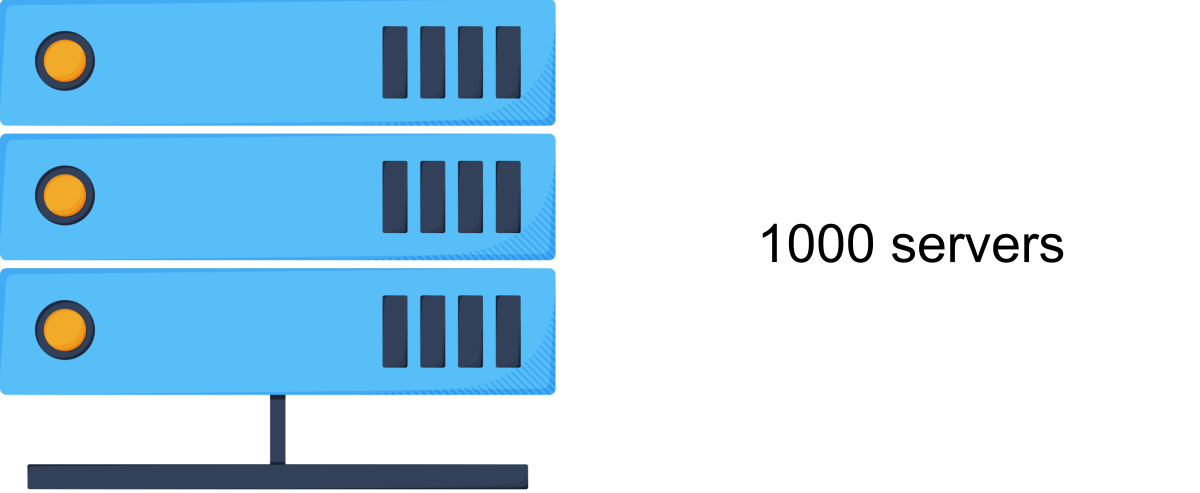
\includegraphics[width=0.25\textwidth]{Images/chapter_29/section_4552284171665408/4662755749920768.png}
 \caption{The number of servers required for Yelp}
\end{figure}

\subsubsection{Storage estimation}\label{r6cbN6THL4pvBOMWvDTX8}
\\
Let's calculate the storage we need for our data. Let's make the following assumptions:

\begin{itemize}
\item
\protect\phantomsection\label{GPF4_52Q7KydExC9VXlar}
We have a total of 500 million places.
\item
\protect\phantomsection\label{IepWItVra5zC7eotFUwoS}
For each place, we need 1,296 Bytes of storage.
\item
\protect\phantomsection\label{QjdxHa3gmy16p2KY-yqSL}
We have one photo attached to each place, so we have 500 million photos.
\item
\protect\phantomsection\label{JMjpgedmJpi22mHN4qn-u}
For each photo, we need 280 Bytes of storage. Here , we consider the row size of the photo entity in the table, which contains a link to the actual photo in the blob store.
\item
\protect\phantomsection\label{P8289thx4TRPGzBkvKjup}
At least 1 million reviews of different places are added daily.
\item
\protect\phantomsection\label{oVhBSCH0E902IK9tdxsyI}
For each review, we need 537 Bytes of storage.
\item
\protect\phantomsection\label{dGdFHvYnZFQ8pFSyYwflD}
We have a total of 178 million users.
\item
\protect\phantomsection\label{F4ykYsVkq5Bh-69SpvGtQ}
For each user, we need 264 Bytes of storage.
\end{itemize}
\begin{quote}
\textbf{Note:} The Bytes used for each place, photo, review, and user are based on the database schema that we'll discuss in the next lesson.
\end{quote}
\\
The following calculator computes the total storage we need:

\begin{figure}[htbp]
 \centering
 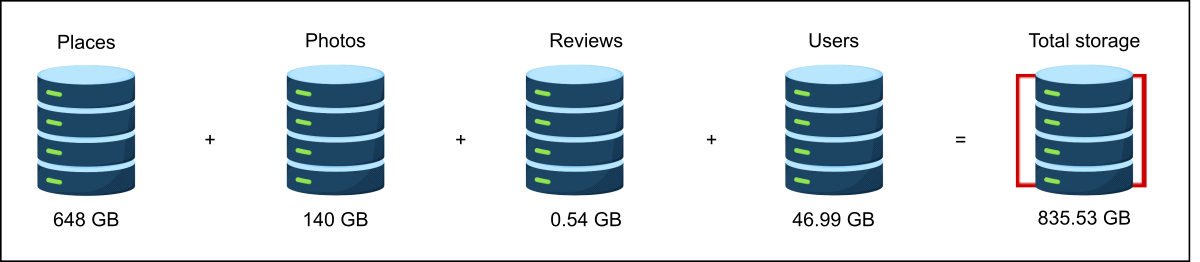
\includegraphics[width=0.5\textwidth]{Images/chapter_29/section_4552284171665408/5998074403356672.png}
 \caption{The total amount of storage required by Yelp}
\end{figure}

\begin{quote}
\textbf{Note:} For reviews, the estimate of 0.54 GB represents only a single day\textquotesingle s reviews. For long-term storage over 10 years, we need to multiply this by the number of days (365×10), giving us approximately 2 TB, which is a more realistic storage requirement. This will also increase the total storage to approximately 2.8 TB.
\end{quote}
\subsubsection{Bandwidth estimation}\label{Oze5EhXEY0zQ-LsP1aGol}
\\
To estimate the bandwidth requirements for Yelp, we categorize the bandwidth calculation of incoming and outgoing traffic.
\\
For incoming traffic, let's assume the following:

\begin{itemize}
\item
\protect\phantomsection\label{UsZHKRyJQcarKqtvePiEm}
On average, five places are added every day.
\item
\protect\phantomsection\label{DP1QglsPA1NuFTV1xpcuD}
For each place, we take up 1,296 Bytes.
\item
\protect\phantomsection\label{gIYqo2mKUGdHIi5QaQ-jY}
A photo of size 3 MB is also attached with each place. This is the size of the photo that we save in the blob store.
\item
\protect\phantomsection\label{aRFPp4WYjP53WRLVWsOxM}
One million reviews of different places are added every day.
\item
\protect\phantomsection\label{ksbUeZ3bNhENNp0Go2IxZ}
Each review, takes up 537 Bytes.
\end{itemize}
\\
We divide the total size of information per day by 86,400 to convert it into per second bandwidth.


For outgoing traffic, let's assume the following:

\begin{itemize}
\item
\protect\phantomsection\label{QJkZ4hMidh6sAPptfC0C3}
A single search returns 20 places on average.
\item
\protect\phantomsection\label{9SXgX7z0Fv9O9Gtn0o_8E}
Each place has a single photo attached to it that has an average size of 3 MB.
\item
\protect\phantomsection\label{HwmheA59VzzTTtLcjJbkN}
Every returned entry contains the place and photo information.
\end{itemize}
\\
Considering that there are 60 million active daily users, we come to the following estimations:


We need a total of approximately \protect\phantomsection\label{katex_inline_RNVaorMV9pUj4Lf6xd646}{{{\(51\ \text{Kbps}\)}}} of incoming traffic and approximately \protect\phantomsection\label{katex_inline_z1l3wu8AfMUUcgdJHfMY_}{{{\(331\ \text{Gbps}\)}}} of outgoing, assuming that the uploaded content is not compressed.\\
\strut \\
Total bandwidth requirements = \protect\phantomsection\label{katex_inline_I6dr1CoKVSgKlyT5E2ZyO}{{{\(51\ \text{Kbps} + 331\ \text{Gbps} \approx 331\ \text{Gbps}\)}}}.\\

\begin{figure}[htbp]
 \centering
 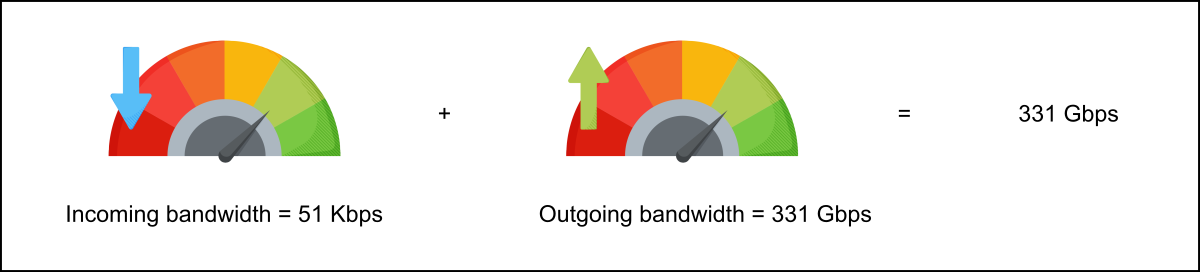
\includegraphics[width=0.5\textwidth]{Images/chapter_29/section_4552284171665408/6100253353050112.png}
 \caption{The total bandwidth required by Yelp}
\end{figure}

\subsection{Building blocks we will use}\label{s8eYUjmzXqIL11DQmqYjW}
\\
The design process of Yelp utilizes many building blocks that have already been discussed in the initial chapters of the course. We 'll consider the following concepts while designing Yelp:

\begin{figure}[htbp]
 \centering
 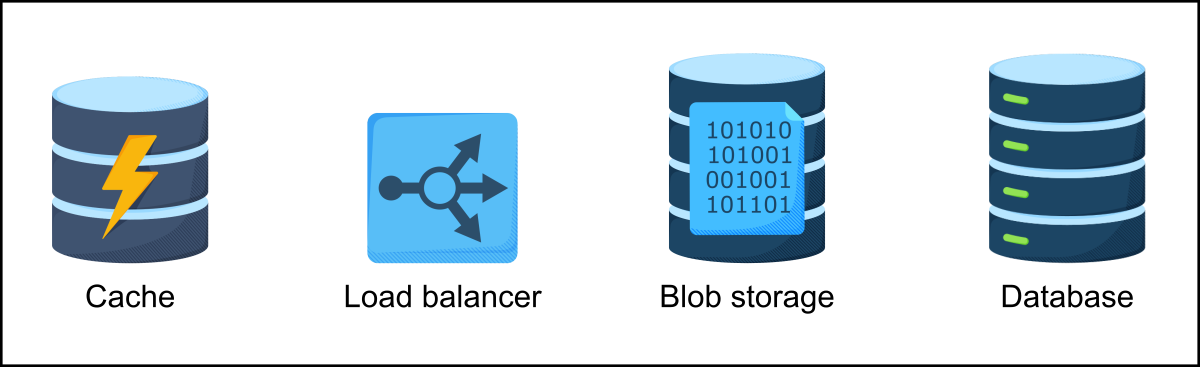
\includegraphics[width=0.5\textwidth]{Images/chapter_29/section_4552284171665408/5007514519601152.png}
 \caption{Building blocks in the high-level design of Yelp}
\end{figure}

\begin{itemize}
\item
\protect\phantomsection\label{ItSy2ffW0wNSQ6rJmsk6Y}
\href{https://www.educative.io/courses/grokking-the-system-design-interview/system-design-the-distributed-cache}{\textbf{Caching}}: We'll use the cache to store information about popular places.
\item
\protect\phantomsection\label{U0FN90Fhn__C8yx8BXxuE}
\href{https://www.educative.io/courses/grokking-the-system-design-interview/introduction-to-load-balancers}{\textbf{Load balancer}}: We'll use the load balancer to manage the large number of requests.
\item
\protect\phantomsection\label{eRKQB4LamVDGwQXrffddu}
\href{https://www.educative.io/courses/grokking-the-system-design-interview/system-design-a-blob-store}{\textbf{Blob storage}}: We'll store images in the blob storage.
\item
\protect\phantomsection\label{QhBXZJiJT7pAu5E8BWbs-}
\href{https://www.educative.io/courses/grokking-the-system-design-interview/introduction-to-databases}{\textbf{Database}}: We'll store information about places and users in the database.
\end{itemize}
\\
We'll also rely on \href{https://www.educative.io/courses/grokking-the-system-design-interview/system-design-google-maps}{\textbf{Google Maps}} to understand the feature of searching for places within a particular radius.

% End of section content